\section{Ring-Like Structures} 

  We have extensively talked about groups, and now we look at an algebraic structure called a ring that has two operations. As we introduce rings, we will use the integers as the primary structure to demonstrate our theorems, along with the ring of continuous functions and the ring of matrices. 

  \begin{definition}[Ring]
    A \textbf{ring} is a set $(R, +, \times)$ equipped with two operations, called addition and multiplication. It has properties: 
    \begin{enumerate}
      \item $R$ is an abelian group with respect to $+$, where we denote the additive identity as $0$ and the additive inverse of $x$ as $-x$. 
      \item $R$ is a monoid with respect to $\times$, where we denote the multiplicative identity as $1$, also known as the \textbf{unity}. 
      \item $\times$ is both left and right distributive with respect to addition $+$
      \begin{align}
        a \times (b + c) & = a\times b + a\times c \\ 
        (a + b) \times c & = a\times c + b\times c 
      \end{align}
      for all $a, b, c \in \mathbb{R}$. 
    \end{enumerate} 
    If $\times$ is associative, $R$ is called an \textbf{associative ring}, and if $\times$ is commutative, $R$ is called a \textbf{commutative ring}. 
  \end{definition}

  In fact, in some cases the existence of the multiplicative identity is not even assumed, though we will do it here.\footnote{If a multiplicative identity is not assumed, then this is called an \textit{rng}, or a \textit{rung}.} Since a ring is a group with respect to addition, we know from \ref{thm:unique_add_inverse} that additive inverses are unique. However, we can say a little more with rings because of the distributive property. 

  \begin{lemma}[Additive Inverses] 
    For any $a \in R$, $-a = -1 \times a$. 
  \end{lemma}
  \begin{proof}
    We can see that 
    \begin{align}
      -1 + 1 = 0 & \implies (-1 + 1) \times a = 0 \times a \\
                 & \implies -1 \times a + 1 \times a = 0 \\
                 & \implies -1 \times a + a = 0 
    \end{align}
    and therefore by definition $-1 \times a$ must be the additive inverse. 
  \end{proof} 

  It helps to see some familiar examples of rings first before examining their properties. 

  \begin{example}[Integers, Rationals, Reals, Complexes]
    $(\mathbb{Z}, +, \times)$, $(\mathbb{Q}, +, \times)$, $(\mathbb{R}, +, \times)$, $(\mathbb{C}, +, \times)$ are all commutative rings, with additive and multiplicative identities $0$ and $1$. 
  \end{example}

  \begin{example}[Matrices]
    The set of matrices $\mathbb{R}^{n \times n}$\footnote{really over any field and even more generally a ring $R$} forms a noncommutative ring under matrix addition $+$ and multiplication $\times$. It has the additive and multiplicative identities $0$ and $I_{n}$. This forms a non-commutative ring for $n > 1$, even when $R$ is commutative.
  \end{example}

  \begin{example}[Continuous Functions]
    The set of all continuous functions $f: \mathbb{R} \rightarrow \mathbb{R}$ is a ring under point-wise addition and multiplication. 
  \end{example}

  \begin{example}[Power Set]
    Given a set $X$, $(2^X, \bigtriangleup, \cap)$ is a commutative associative ring with respect to the operations of symmetric difference $M \bigtriangleup N \coloneqq (M \setminus N) \cup (N \setminus M)$ and intersection. The additive identity is $\emptyset$ and the multiplicative identity is $X$. We can clearly see that both operations are commutative and $\cap$ is associative. 
    \begin{align*}
      M \bigtriangleup N & = (M \setminus N) \cup (N \setminus M) \equiv N \bigtriangleup M \\
      M \cap N & = N \cap M \\
      M \cap N \cap P & = (M \cap N) \cap P = M \cap (N \cap P)
    \end{align*}
  \end{example}

  Next, just like how we did for groups, we can talk about subrings. 

  \begin{definition}[Subring]
    Given ring $(R, +, \times)$ a \textbf{subgring} $(S, +, \times)$ is a ring such that $S \subset R$. $S$ is called a \textbf{proper subring} if $S \subsetneq R$. 
  \end{definition}

  \begin{theorem}
    If $S_1, S_2$ are subrings of $R$, then $S_1 \cap S_2$ is a subring. 
  \end{theorem}

  Note that we do not assume that there exists multiplicative inverses in a ring. However, there may be some elements for which multiplicative inverses do exist, i.e. $a, b \in R$ where $ab = 1$.  

  \begin{definition}[Unit]
    A \textbf{unit} of a ring $R$ is an element $u \in R$ that has a multiplicative inverse in $R$. That is, there exists a $v \in R$ s.t. $uv = vu = 1$. 
  \end{definition}

  Another property that we would desire is some sort of decomposition of ring elements as other ring elements. More specifically, the existence of elements $a, b$ such that $ab = 0$ will be of particular interest to us. 

  \begin{definition}[Left, Right Divisor]
    Let $a, b, r \in R$ a ring. 
    \begin{enumerate}
      \item If $ab = r$, then $a$ is said to be a \textbf{left divisor} of $r$ and $b$ a \textbf{right divisor} of $r$. 

      \item $a$ is said to be a left divisor of $r$ if it is a left divisor and a right divisor of $r$: $ax = ya = r$, but $x$ does not necessarily equal $y$. 

      \item If $ab = 0$, then $a$ and $b$ are said to be a \textbf{left zero divisor} and \textbf{right zero divisor}, respectively. 
    \end{enumerate}
    If $R$ is commutative, then we just call $a$ a \textbf{divisor} of $r$ or a \textbf{zero divisor}.\footnote{$a$ is a right divisor of $b \iff \exists x (xa = b) \iff \exists x (ax = b) \iff a$ is a left divisor. } 
  \end{definition}

  It turns out that the existence of units and zero divisors classify rings into subcategories, which we will elaborate on. That is, we will start with the most general theory on rings, and then shrink down into subcategories of rings. 

  \begin{figure}[H]
    \centering 
    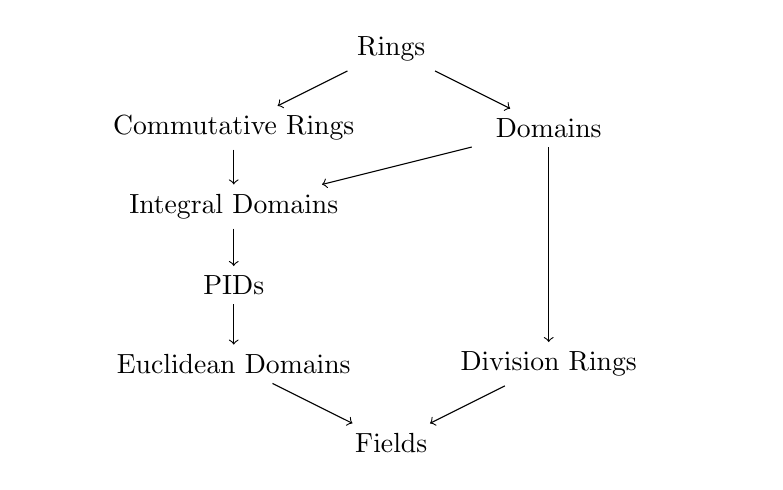
\begin{tikzpicture}[
        node distance=2cm,
        box/.style={
            text width=5cm,
            align=center
        }
    ]
        % Nodes for ring types
        \node[box] (rings) at (0,0) {Rings};
        \node[box] (comm) at (-2,-1) {Commutative Rings};
        \node[box] (domains) at (2,-1) {Domains};
        \node[box] (int) at (-2,-2) {Integral Domains};
        \node[box] (divring) at (2,-4) {Division Rings};
        \node[box] (pid) at (-2,-3) {PIDs};
        \node[box] (euc) at (-2,-4) {Euclidean Domains};
        \node[box] (fields) at (0,-5) {Fields};
        
        % Left path arrows
        \draw[->] (rings) -- (comm);
        \draw[->] (comm) -- (int);
        \draw[->] (int) -- (pid);
        \draw[->] (pid) -- (euc);
        \draw[->] (euc) -- (fields);
        \draw[->] (divring) -- (fields);
        
        % Right path arrows
        \draw[->] (rings) -- (domains);
        \draw[->] (domains) -- (int);
        \draw[->] (domains) -- (divring);
    \end{tikzpicture}
    \caption{Basic hierarchy of rings.} 
    \label{fig:ring_hierarchy}
  \end{figure} 

  Finally, we will mention a product ring. 

  \begin{definition}[Direct Product of Rings]
    Given rings $(R, +_R, \times_R)$ and $(S, +_S, \times_S)$, the direct product of the rings is the set $R \times S$ with the operations 
    \begin{enumerate}
      \item $(r_1, s_1) + (r_2, s_2) \coloneqq (r_1 +_R r_2, s_1 +_S s_2)$. 
      \item $(r_1, s_1) \times (r_2, s_2) \coloneqq (r_1 \times_R r_2, s_1 \times_S s_2)$. 
    \end{enumerate}
    This is indeed a ring. 
  \end{definition}

\subsection{Ring Homomorphisms}

  So far, we have talked about many properties of rings but have not thoroughly gone over their classification. This is what we will do in this section, just like how we have classified groups. It turns out that classifying rings is significantly harder to do so, so we will talk about some low-order finite rings and provide some examples of isomorphisms between more complex rings. 

  \begin{definition}[Ring Homomorphism, Isomorphism]
    A \textbf{ring homomorphism} $f: R \rightarrow S$ is a function that satisfies for all $a, b \in R$
    \begin{enumerate}
      \item $f(a + b) = f(a) + f(b)$
      \item $f(ab) = f(a) f(b)$ 
      \item $f(1_R) = 1_S$\footnote{The reason we need this third is that while $f$ is a group homomorphism with respect to $+$, it automatically follows that $f(0) = 0$. However $f$ is only a monoid homomorphism w.r.t. $\times$, and so we need this extra constraint. }
    \end{enumerate}
    for all $a, b \in R$.\footnote{Note that the first is equivalent to it being a group homomorphism between $(R, +)$ and $(S, +)$. The second property may look like it is a group homomorphism between $(R, \times)$ and $(S, \times)$, but remember that neither are groups and it just states that closure distributes. Combined with the fact that the multiplicative identity matches, $f$ is really a homomorphism of \textit{monoids}. } Furthermore, 
    \begin{enumerate}
      \item A \textbf{ring isomorphism} is a bijective ring homomorphism, and we call rings $R$ and $S$ isomorphic, denoted $R \simeq S$ if there exists an isomorphism between them. 
      \item A \textbf{ring endomorphism} is a ring homomorphism onto itself. 
      \item A \textbf{ring automorphism} is an isomorphism from a ring to itself. 
    \end{enumerate}
  \end{definition} 

  \begin{example}[Homomorphisms of Rings]
    We provide some simple examples of ring homomorphisms. 
    \begin{enumerate}
      \item The identity map $\iota : R \to R$ is a ring homomorphism. 
      \item If $R \subset S$ as rings, then the canonical injection map $\iota: R \to S$ is a ring homomorphism. 
      \item Complex conjugation $z \in \mathbb{C} \mapsto \bar{z} \in \mathbb{C}$ is a ring automorphism. 
    \end{enumerate}
  \end{example} 

  \begin{definition}[Kernel]
    The \textbf{kernel} of a ring homomorphism $f: R \rightarrow S$ is the preimage of $0 \in S$.\footnote{Note that this is the additive identity, not the multiplicative identity. We must specify which identity, unlike a group which has just one identity.}
  \end{definition}

  \begin{lemma}[Images and Kernels of Ring Homomorphisms]
    If $f: R \rightarrow S$ is a ring homomorphism, then 
    \begin{enumerate}
      \item $\ker{f}$ is a subring of $R$. 
      \item $\im{f}$ is a subring of $S$. 
      \item $f$ is injective iff $\ker{f} = \{0\}$. 
    \end{enumerate}
  \end{lemma}
  \begin{proof}

  \end{proof}

  \begin{theorem}[Compositions of Ring Homomorphisms]
    Compositions of ring homomorphisms are ring homomorphisms. 
  \end{theorem} 
  \begin{proof}
    
  \end{proof}

  Now let's focus a bit more on ring isomorphisms. The following should be intuitive. 

  \begin{lemma}[Properties of Ring Isomorphisms]
    If $f$ is a ring isomorphism, then $f^{-1}$ is a ring isomorphism. 
  \end{lemma} 

\subsection{Commutative Rings} 

  Remember that for commutative rings, distinguishing left and right divisors are meaningless, and so we can talk about just \textit{divisors}. Almost all rings that we will deal with are commutative, so let's try to find some properties of commutative rings.  

  \begin{definition}[Prime and Compositive Elements]
    In a commutative ring $R$, an element $p \in R$ is said to be \textbf{prime} if it is not $0$, not a unit, and has only divisors $1$ and $p$. 
  \end{definition}

  \begin{lemma}[Euclid]
    If $p$ is prime, then $p \mid ab \implies p \mid a$ or $p \mid b$.  
  \end{lemma}

  \begin{lemma} 
    Let $R$ be a commutative ring and $a, b, d \in R$. If $d \mid a$ and $d \mid b$, then $d \mid (ma + nb)$ for any $m, n \in R$. 
  \end{lemma} 

  \begin{definition}[Greatest Common Divisor]
    The \textbf{greatest common divisor} of elements $a$ and $b$, denoted $\gcd(a, b)$ of an commutative ring $R$ is a common divisor of $a$ and $b$ divisible by all their common divisors. That is, it is the element $d \in R$ satisfying 
    \begin{enumerate}
      \item $d \mid a$ and $d \mid b$ 
      \item if $k \mid a$ and $k \mid b$, then $k \mid d$. 
    \end{enumerate}
    If $\mathrm{gcd}(a, b) = 1$, then $a$ and $b$ are said to be \textbf{relatively prime}. 
  \end{definition} 

  Note that in an arbitrary commutative ring, the gcd of two elements always exists since we can at least identify $1$, but there may not be a \textit{unique} gcd. 

\subsection{Domains}

  We can see that domains behave similarly to the integers, but with the missing property that $\times$ is commutative. This motivates the following definition of an integral domain, which can be seen as a generalization of the integers. 

  \begin{definition}[Domain, Integral Domain]
    A ring $R$ with no zero divisors for every element is called a \textbf{domain}. An \textbf{integral domain} is a commutative domain $R$.\footnote{Almost always, we work with integral domains so we will default to this.} 
  \end{definition} 

  \begin{example}[Domains vs Integral Domains]
    We show some examples of domains and integral domains. 
    \begin{enumerate}
      \item $(\mathbb{Z}, +, \times)$ is an integral domain
      \item $(\mathbb{Q}, +, \times)$ is an integral domain. 
      \item $(\mathbb{R}, +, \times)$ is an integral domain. 
      \item Quaternions $\mathbb{H}$ are not commutative but are a domain. 
    \end{enumerate}
  \end{example} 

  \begin{example}[Non-Domains]
    Here are some examples of non-domains. 
    \begin{enumerate}
      \item The ring of $n \times n$ matrices over any nonzero ring when $ n \geq 2$ is not a domain. Given matrices $A, B$, if the image of $B$ is in the kernel of $A$, then $A B = 0$.
      \item The ring of continuous functions on the interval is not a domain. To see why, notice that given the piecewise functions 
      \begin{equation}
        f (x) = \begin{cases}
        1 - 2x & x \in [0, \frac{1}{2}] \\
        0 & x \in [\frac{1}{2}, 1] 
        \end{cases}, \; \;\;g (x) = \begin{cases}
        0 & x \in [0, \frac{1}{2}] \\
        2x - 1 & x \in [\frac{1}{2}, 1] 
        \end{cases}
      \end{equation}
      $f, g \neq 0$, but $f g = g f = 0$. 

      \item A product of two nonzero commutative rings with unity $R \times S$ is not an integral domain since $(1,0) \cdot (0, 1) = (0, 0) \in R \times S$. 
    \end{enumerate}
  \end{example}

  Here is an alternative equivalent characterization of an integral domain. 

  \begin{definition}[Regular Elements]
     An element $r$ of a ring $R$ is \textbf{regular} if the mapping 
     \begin{equation}
       \rho: R \longrightarrow R, \qquad x \mapsto x r
     \end{equation}
    is injective for all $x \in R$. 
  \end{definition}

  \begin{theorem}[Integral Domains w.r.t. Regularity]
    An integral domain is a commutative associative ring where every element is regular. 
  \end{theorem} 

  Finally, we talk about the properties of integral domains. Namely, that the characteristic must be prime and that gcd's---while not yet unique---are now guaranteed to be \textit{associated}. 

  \begin{theorem}[Characteristic of an Integral Domain]
    The characteristic of an integral domain is either $0$ or a prime number. 
  \end{theorem}

  While we have shown that gcd's exist in commutative rings, we can say a bit more when working in Euclidean domains. 

  \begin{definition}[Associate Elements]
    Elements $a$ and $b$ are \textbf{associated}, denoted $a \sim b$ if either of the following equivalent conditions holds
    \begin{enumerate}
        \item $a | b \text{ and } b | a$
        \item $a = c b, \text{ where } c$ is invertible
    \end{enumerate}
    The two conditions are equivalent because $c$ and $c^{-1}$ are both in $A$. 
  \end{definition} 

  \begin{theorem}[GCD's in a Euclidean Domain]
    Any two distinct gcd's of $a, b$ in a Euclidean domain must be associate elements. 
  \end{theorem}

\subsection{Ideals}

  Now assuming that $R$ and $S$ are commutative rings, let's consider a special sort of subset of a commutative ring. Consider the kernel of the ring homomorphism. We can see that if $a, b \in \ker(f)$, then $f(a + b) = f(a) + f(b) = 0 + 0 = 0$, and so $\ker(f)$ is closed under addition. Furthermore, $a \in \ker(f)$ and \textit{any} $b \in R$ gives $f(ab) = f(a) f(b) = 0 f(b) = 0$, and so multiplying any element in the kernel by an arbitrary element in the rings keeps it in the kernel. We would like to generalize these properties into an \textit{ideal}. 

  \begin{definition}[Ideals]
    For a commutative ring $(R,+, \times)$, a \textbf{two-sided ideal}---or \textbf{ideal}---is a subset $I \subset R$ satisfying 
    \begin{enumerate}
      \item $(I, +)$ is a subgroup of $(R, +)$. 
      \item $a \in I, r \in R \implies ra = ar \in I$.\footnote{Note that this property and closure under addition actually implies that it is a subgroup. Since we can see that $-1 \in R$ and $a \in I$ implies $-1 \cdot a = -a \in I$.}
    \end{enumerate}
    If $R$ is not necessarily commutative, then we $ra \neq ar$ in general, so we may distinguish between left and right ideals. 
  \end{definition}

  Therefore, we can see that it is an abelian group under $+$ and closed under $\times$. However, it is not guaranteed to have a multiplicative identity, which is why we can interpret $I$ as a ring without a multiplicative identity, also known as a \textit{rung}. 

  This seems like a pretty abstract definition, but a good intuition to have---though not completely accurate---is that ideals are a collection of \textit{multiples} of a certain element.\footnote{This is actually more accurate for a principal ideal.} They are analogous to normal subgroups, which were used to induce a congruence relation on a group to get its quotient. Ideals play a similar role. 

  \begin{example}[Multiples of Elements Are an Ideal]
    We give 2 ideals: 
    \begin{enumerate}
      \item The set of even integers $2 \mathbb{Z}$ is an ideal in the ring $\mathbb{Z}$, since the sum of any even integers is even and the product of any even integer with an integer is an even integer. However, the odd integers do not form an ideal. 
      \item The set of all polynomials with real coefficients which are divisible by the polynomial $x^2 + 1$ is an ideal in the ring of all polynomials. 
    \end{enumerate}
  \end{example}

  Let's talk about a few more properties of ideals, namely their construction and behavior under set theoretic operations. 

  \begin{theorem}[Sum and Intersection of Ideals are Ideals] 
    \label{thm:sum_int_ideals}
    Given two ideals $I, J \subset R$, 
    \begin{enumerate}
      \item $I \cap J$ is an ideal. 
      \item $I + J \coloneqq \{i + j \mid i \in I, j \in J\}$ is an ideal. 
    \end{enumerate}
  \end{theorem}
  \begin{proof}
    Listed. 
    \begin{enumerate}
      \item $I \cap J$ is an ideal. Given $a, b \in I \cap J$, then $a, b \in I \implies a + b \in I$, and $a, b \in J \implies a + b \in J$. So $a + b \in I \cap J$. Furthermore, for every $r \in R$, $a \in I \implies r a \in I$ and $a \in J \implies r a \in J$, so $a \in I \cap J \implies ra \in I \cap J$. 

      \item $I + J$ is an ideal. Given $x, y \in I + J$, then $x = a_x + b_x$ and $y = a_y + b_y$ for $a_x, a_y \in I, b_x, b_y \in J$. So 
      \begin{equation}
        x + y = (a_x + b_x) + (a_y + b_y) = (a_x + a_y) + (b_x + b_y)
      \end{equation}
      where $a_x + a_y \in I, b_x + b_y \in J$ by definition of an ideal, and so $x + y \in I + J$. Noe let $x = a_x + b_x \in I + J$. Then given $r \in R$,
      \begin{equation}
        rx = r(a_x + b_x) = r a_x + r b_x
      \end{equation}
      where $r a_x \in I$ and $r b_x \in J$ since $I, J$ are ideals. Therefore $rx \in I + J$.  
    \end{enumerate}
  \end{proof}
  
  \begin{theorem}[Preimage of Ideals are Ideals]
    If $f: R \to S$ is a ring homomorphism of commutative rings $J \subset S$ is an ideal, then $f^{-1} (J)$ is an ideal of $R$. 
  \end{theorem}
  \begin{proof}
    
  \end{proof}

  \begin{example}[Image of Ideal is Not Necessarily an Ideal]
    It is not true in general that for an ideal $I \subset R$ and a ring homomorphism $f: R \to S$, the image $f(I)$ is an ideal of $S$. 
  \end{example}

  Given the two examples above, let's formalize the idea of an ideal consisting of all multiples of a specific element $a$. This sounds pretty familiar to \textit{generators} of groups. 

  \begin{definition}[Generators of Ideals]
    Given a commutative ring $R$, the \textbf{ideal generated by $a \in R$} is denoted 
    \begin{equation}
      \langle a \rangle \coloneqq \{r a \mid r \in R\}
    \end{equation}
    and more generally, we may have multiple generating elements. 
    \begin{equation}
      \langle a_1, \ldots, a_n \rangle \coloneqq \{ r_1 a_1 + \ldots r_n a_n \mid r_1, \ldots, r_n \in R \}
    \end{equation}
  \end{definition}

  Therefore, the ideals considered above can be written $\langle 2 \rangle \subset \mathbb{Z}$ and $\langle x - 2 \rangle \subset \mathbb{Q}[x]$. However, it may be the case that two elements generate the same ideal in a non-Euclidean domain, but constructing such an example is a bit challenging.   

  \begin{example}[Matrix with Last Row of Zeros]
    Let $R$ be the set of all $n \times n$ matrices. Then 
    \begin{enumerate}
      \item The set of all $n \times n$ matrices whose last row is zero forms a right ideal, but not a left ideal.
      \item The set of all $n\times n$ matrices whose last column is zero is a left ideal, but not a right ideal. 
    \end{enumerate}
  \end{example}

\subsection{Quotient Rings}

  What is nice about ideals is that they induce not just an equivalence relation---but a congruence relation---on a ring, which is a generalization of working in the integers modulo $n$. 

  \begin{theorem}[Equivalence Relation Induced by an Ideal]
    Given a commutative ring $R$ and an ideal $I \subset R$, we say that two elements $a, b \in R$ are \textbf{congruent} $\pmod{I}$, written $a \equiv b \pmod{I}$ iff $a - b \in I$. We claim two things: 
    \begin{enumerate}
      \item $\equiv$ is an equivalence relation. 
      \item $\equiv$ is a congruence relation. Given that $a \equiv a^\prime \pmod{I}$ and $b \equiv b^\prime \pmod{I}$, 
      \begin{equation}
        a + b \equiv a^\prime + b^\prime \pmod{I}, \qquad ab \equiv a^\prime b^\prime \pmod{I}
      \end{equation}
    \end{enumerate}
    Occasionally, if the ideal $I$ is clear from context, we will write $a \equiv b$. 
  \end{theorem}
  \begin{proof}
    We first prove that $\equiv$ is indeed an equivalence relation. 
    \begin{enumerate}
      \item \textit{Reflexive}. $a \equiv a \pmod{I}$ is trivial since $a - a = 0 \in I$. 
      \item \textit{Symmetric}. If $a \equiv b$, then $a - b \in I \implies -(a - b) = -a + b = b - a \in I \implies b \equiv a$. 
      \item \textit{Transitive}. If $a \equiv b$ and $b \equiv c$, then $a - b \in I$ and $b - c \in I$. Since $I$ is an additive group and so it is closed under addition, so $(a - b) + (b - c) = a - c \in I \implies a \equiv c$. 
    \end{enumerate}
    Note that so far, we have only used the group property of ideals to prove that is is an equivalence class. Now for congruence of multiplication, we need the ring properties. 
    \begin{enumerate}
      \item $a \equiv a^\prime, b \equiv b^\prime \implies (a - a^\prime), (b - b^\prime) \in I$. By adding them together and distributivity, we have 
      \begin{equation}
        a - a^\prime + b - b^\prime = (a + b) - (a^\prime + b^\prime) \in I \implies a + b \equiv a^\prime + b^\prime \pmod{I}
      \end{equation}

      \item We see that $a \in R, (b - b^\prime) \in I \implies a(b - b^\prime) \in I$. Similarly, $b^\prime \in R, (a - a^\prime) \in I \implies (a - a^\prime) b^\prime \in I$. Now adding the two, we have 
      \begin{equation}
        a (b - b^\prime) + (a - a^\prime) b^\prime = ab - ab^\prime + ab^\prime - a^\prime b^\prime = ab - a^\prime b^\prime \in I \implies ab = a^\prime b^\prime \pmod{I}
      \end{equation}
    \end{enumerate}
  \end{proof} 

  This quotient space maintains a lot of nice properties of the algebraic operations, and so we can form a new ring structure with this quotient space.  

  \begin{definition}[Quotient Rings, Rings of Residue Class]
    The quotient space $R/I$ induced by the mapping $a \mapsto [a]$ is indeed a commutative ring, called the \textbf{quotient ring}, with addition and multiplication defined 
    \begin{equation}
      [a] + [b] \coloneqq [a + b], \qquad [ab] \coloneqq [a] \, [b]
    \end{equation}
  \end{definition}
  \begin{proof}
    Note that the properties of the operation in $\frac{M}{R}$ inherits all the properties of the addition operation on $M$ that are expressed in the form of identities and inverses, along with the existence of the zero identity. 
    \begin{align*}
      0 \in M & \implies [0] \text{ is the additive identity in } \frac{M}{R} \\
      a + (-a) = 0 & \implies [a] + [-a] = [0] \\
      1 \in M & \implies [1] \text{ is the multiplicative identity in } \frac{M}{R}
    \end{align*}
  \end{proof} 

  \begin{theorem}[Quotient Maps are Homomorphisms]
    The map $p: R \to R/I$ is a ring homomorphism. 
  \end{theorem}
  \begin{proof}
    This is true by definition since we have made $\equiv$ a congruence relation. 
  \end{proof}

  \begin{example}[Quotient Rings of Integers]
    The quotient set $\mathbb{Z}/\langle n \rangle$ by the relation of congruence modulo $n$ is denoted $\mathbb{Z}_{n}$. 
    \begin{equation}
      \mathbb{Z}_{n} = \{ [0]_{n}, [1]_{n}, \ldots, [n-1]_{n} \}
    \end{equation}
    Note that the quotient ring $(\mathbb{Z}/\langle n \rangle, +, \times)$ is precisely the cyclic quotient group $\mathbb{Z}_n = \mathbb{Z}/6\mathbb{Z}$ when considering only addition. We list some quotient rings of the integers. 
    \begin{enumerate}
      \item In $\mathbb{Z}_{5} = \mathbb{Z}/\langle 5 \rangle$, the elements $[2]$ and $[3]$ are multiplicative inverses of each other since $[2] [3] = [6] = [1]$, and $[4]$ is its own inverse since $[4] [4] = [16] = [1]$. The addition and multiplication tables for $\mathbb{Z}_5$ is shown below. 
      \item Consider the ideal $I = \langle 2 \rangle \subset \mathbb{Z}_6$. We have $0 \equiv 2 \equiv 4 \pmod{I}$ and $1 \equiv 3 \equiv 5 \pmod{I}$, and so the quotient ring $\mathbb{Z}_6 / I$ consists of the two equivalence classes $[0]$ and $[1]$. 
    \end{enumerate}
  \end{example}

  \begin{example}[Quotient Rings of Polynomials]
    We list some quotient rings of polynomials. 
    \begin{enumerate}
      \item Consider $\mathbb{Q}[x] / \langle x^2 - 2 \rangle$. We can see that any polynomial $f \in \mathbb{Q}[x]$ is equivalent $\pmod{I}$ to a linear polynomial, since $x^2 \equiv 2$. Alternatively we can apply the division algorithm to replace $f(x)$ by its remainder upon division by $x^2 - 2$, and thus in the quotient ring, $[x]$ plays the role of $\sqrt{2}$, which may indicate that $\mathbb{Q}[x] / \langle x^2 - 2 \rangle = \mathbb{Q}[\sqrt{2}]$. 
      \item Consider $\mathbb{Z}_2 [x]/ \langle x^2 + x + 1 \rangle$. As in the previous example, any polynomial in $\mathbb{Z}_2[x]$ is equivalent to a linear polynomial since $x^2 \equiv x + 1 \pmod{I}$. Therefore the elements of the quotient ring are $[0], [1], [x], [x+1]$ with the addition and multiplication tables. 

      \begin{figure}[H]
        \centering
        \begin{subfigure}[b]{0.48\textwidth}
          \centering
          \begin{tabular}{c|cccc}
            $+$ & $0$ & $1$ & $x$ & $x + 1$ \\
            \hline
            $0$ & $0$ & $1$ & $x$ & $x + 1$ \\
            $1$ & $1$ & $0$ & $x + 1$ & $x$ \\
            $x$ & $x$ & $x + 1$ & $0$ & $1$ \\
            $x + 1$ & $x + 1$ & $x$ & $1$ & $0$ \\
          \end{tabular}
          \caption{}
        \end{subfigure}
        \hfill 
        \begin{subfigure}[b]{0.48\textwidth}
          \centering
          \begin{tabular}{c|cccc}
            $\cdot$ & $0$ & $1$ & $x$ & $x + 1$ \\
            \hline
            $0$ & $0$ & $0$ & $0$ & $0$ \\
            $1$ & $0$ & $1$ & $x$ & $x + 1$ \\
            $x$ & $0$ & $x$ & $x + 1$ & $1$ \\
            $x + 1$ & $0$ & $x + 1$ & $1$ & $x$ \\
          \end{tabular}
          \caption{}
        \end{subfigure}
        \label{fig:boolean-algebra-tables}
      \end{figure}
    \end{enumerate}
  \end{example}

  Note that just like how quotient topologies do not preserve topological properties, as shown \hyperref[pst-quotient_trivial]{here} and \hyperref[pst-quotient_hausdorff]{here}, quotient rings inherit some---but not all---algebraic properties. 

  \begin{theorem}[Quotient Inherits Commutativity]
    Let $R$ be a commutative ring and $I \subsetneq R$ be an ideal. Then $R/I$ is a commutative ring. 
  \end{theorem}

  \begin{example}[Quotient Does Not Inherit Integral Domain Property]
    $\mathbb{Z}$ is an integral domain, but $\mathbb{Z}/\langle 6 \rangle$ is not since $[2] \times [3] = [0]$. 
  \end{example}

  Just like in group theory, we have a method of constructing isomorphisms between cleverly chosen rings $S$ and a quotient ring $R/I$. This seems to be a common pattern here when considering groups, rings, and topological spaces... This will be investigated more in category theory. 

  \begin{theorem}[Fundamental Ring Homomorphism Theorem]
    Let $R$ and $S$ be commutative rings, and suppose $f: R \rightarrow S$ be a surjective ring homomorphism. Then this induces a ring isomorphism
    \begin{equation}
      R /\ker{f} \simeq S
    \end{equation} 
    satisfying $\phi = \bar{\phi} \circ \pi$. 

    \begin{figure}[H]
      \centering 
      \begin{tikzcd}
        R \arrow[r, "\phi"] \arrow[d, "\pi"] & S \\
        R/\ker(\phi) \arrow[ru, "\bar{\phi}"] &  
      \end{tikzcd}
      \caption{The theorem states that the following diagram commutes. } 
      \label{fig:fund_ring_homo_theorem}
    \end{figure}
  \end{theorem}
  \begin{proof}
    
  \end{proof} 

  A direct application of this is the Chinese remainder theorem. 

  \begin{corollary}[Chinese Remainder Theorem]
    Given a commutative ring $R$, let $I, J \subset R$ be ideals such that $I + J = R$. Then, 
    \begin{equation}
      \pi: R \to \frac{R}{I} \times \frac{R}{J}, \qquad r \mapsto ([r]_I, [r]_J)
    \end{equation}
    with component-wise quotient mappings is a surjective ring homomorphism with $\ker{\pi} = I \cap J$. By the fundamental ring homomorphism theorem, it immediately follows that 
    \begin{equation}
      \frac{R}{I \cap J} \simeq \frac{R}{I} \times \frac{R}{J}
    \end{equation}
  \end{corollary}
  \begin{proof}
    Since $I + J = R$, there exists $i \in I$ and $j \in j$ s.t. $i + j = 1$. Let $\bar{a} = a + I \in R/I$ and $\bar{b} = b + J \in R/J$ be any elements. Then 
    \begin{equation}
      \pi(aj + bi) = ([aj + bi]_I, [a_j + bi]_J) = ([aj]_I, [bi]_J) \in \frac{R}{I} \times \frac{R}{J}
    \end{equation} 
    But we have 
    \begin{enumerate}
      \item $a(j + i) = a \in R \implies aj = a(j + i) \in R/I$. Therefore $[aj]_I = [a]_I$ 
      \item $b(j + i) = b \in R \implies bi = bj + bi \in R/J$. Therefore $[b]_J = [bi]_J$. 
    \end{enumerate}
    Therefore, we have $\pi(aj + bi) = ([a]_I, [b]_J)$, which proves surjectivity. 
  \end{proof} 

  \begin{example}[Chinese Remainder Theorem on Integers]
    
  \end{example} 

  \begin{example}
    We claim that $\mathbb{Z}_{10} \simeq \mathbb{Z}_5 \times \mathbb{Z}_2$ as rings. In fact, the whole isomorphism is defined with the mappings $f(1, 1) = 1$. 
  \end{example}

\subsection{Principal Ideal Domains}

  A good intuition to have about ideals is that they are the set of multiples of a certain element. However, this may not be true for ideals in general, but if this intuition is true, then we call this a \textit{principal ideal}. 

  \begin{definition}[Principal Ideals]
    Given commutative ring $R$ and $I \subset R$, if $I = \langle a \rangle$ for some $a \in R$---i.e. it is generated by a single element---$I$ is called a \textbf{principal ideal}. 
  \end{definition}

  \begin{definition}[Principal Ideal Domain]
    A \textbf{principal ideal domain}, also called a \textbf{PID}, is an integral domain in which every ideal is principal.  
  \end{definition}

  So a principal ideal domain is an integral domain by definition. It may seem that PIDs are an oddly specific structure to be studying separately, but this actually turns out to unlock a lot more nice properties that we are familiar with. The first is that GCDs are now unique, which is great. Second, we have Bezout's identity, saying that if $x$ and $y$ are elements of a PID without common divisors, then every element of the PID can be written in the form $a x + b y$. Finally, and most importantly, any element of a PID has a unique decomposition into irreducible factors. We now introduce some examples of PIDs, which are not as trivial and should be introduced as theorems. 

  \begin{theorem}[Integers and Polynomials over Fields are PIDs]
    The following are all examples of principal ideal domains. 
    \begin{enumerate}
      \item Any field $\mathbb{F}$. 
      \item The ring of integers $\mathbb{Z}$. 
      \item $\mathbb{F}[x]$, rings of polynomials in one variable with coefficients in a field $\mathbb{F}$. 
    \end{enumerate}
  \end{theorem}
  \begin{proof}
    Listed. 
    \begin{enumerate}
      \item It is quite easy to see that a field $\mathbb{F}$ is a PID since the only two possible ideals are $\{0\}$ and $\mathbb{F}$, both of which are principal. 
      \item If $I \subset \mathbb{Z}$ is an ideal, then if $I = \langle 0 \rangle$, then we're done. Otherwise, let $a \in I$ be the smallest positive integer in $I$. It is clear that $\langle a \rangle \subset I$. Now given an element $b \in I$, by the Euclidean algorithm we have $b = aq + r$ with $r < a$. Since $a, b \in I$, it follows that $r \in I$. But since $0 \leq r < a$ and $a$ is the smallest positive integer, $r = 0$, and so $b = aq \implies b \in \langle a \rangle$. 
      \item The ring of polynomials $\mathbb{F}[x]$ is a PID since we can imagine a minimal polynomial $p$ in each ideal $I$. Every element in $I$ must be divisible by $p$, which means that the entire ideal $I$ can be generated by the minimal polynomial $p$, making $I$ principal.  
    \end{enumerate}
  \end{proof}

  \begin{corollary}[Ideals Generated by Primes]
    If $I \subsetneq \mathbb{Z}$ and a prime number $p \in I$, then $I = \langle p \rangle$. If $I \subset F[x]$ is an ideal and irreducible $f(x) \in I$, then $I = \langle f(x) \rangle$. 
  \end{corollary}
  \begin{proof}
    Listed. 
    \begin{enumerate}
      \item Since $\mathbb{Z}$ is a PID, $I = \langle a \rangle$ for some nonzero $a \in \mathbb{Z}$. We can assume $a$ is positive, and if $a = 1$, then $I = \mathbb{Z}$, which contradicts the $I$ is a proper subset. So $a \geq 2$. Now because $p \in I$, $p = ra$ for some $r \in \mathbb{Z}$, but since $p$ is prime, $r = 1, a = p$. 

      \item Since $F[x]$ is a PID and $I = \langle g(x) \rangle$ for some $g(x) \in F[x]$, let us take $f(x) \in I$. Then it must be true that $f(x) = g(x) h(x)$ for some $h(x) \in R$. However, This means that $\deg(g)$ or $\deg(h)$ must be $0$ since $f$ is irreducible. But if $g(x)$ was a constant, then $I = R$, so $g(x) = f(x)$. 
    \end{enumerate}
  \end{proof}

  \begin{corollary}[Kernel of Evaluation Homomorphism is Generated by Irreducible Factor]
    Suppose $f(x) \in F[x]$ is irreducible in $F[x]$, and $K \supset F$ is a field containing a root $\alpha$ of $f(x)$. Then the ideal of all polynomials in $F[x]$ vanishing at $\alpha$ is generated by $f(x)$. That is, given the evaluation homomorphism 
    \begin{equation}
      \ev_\alpha: F[x] \rightarrow K
    \end{equation}
    we claim $\ker(\ev_\alpha) = \langle f(x) \rangle$. 
  \end{corollary}
  \begin{proof}
    This is an immediate consequence of the previous corollary. 
  \end{proof}

  \begin{theorem}[Greatest Common Divisor is Unique in PIDs]
    Given $a, b \in R$ a PID, $\gcd(a, b)$ is unique. 
  \end{theorem}

  \begin{theorem}[Bezout's Theorem]
    Given that one divides (with remainder) polynomial $f$ by $g = x - c$, let the remainder be $r \in F$. That is, 
    \begin{equation}
      f(x) = (x-c) q(x) + r, \; r \in F
    \end{equation}
    This implies that the remainder equals the value of $f$ at point $c$. That is, 
    \begin{equation}
      f(c) = r
    \end{equation}
    Note that a corollary of this is the single factorization theorem, but the single factorization holds for commutative rings in general. 
  \end{theorem} 

  Note that Bezout's does not hold in integral domains in general. 
  
  \begin{example}[Counterexample in Integral Domains but not PIDs]
    
  \end{example}

  \begin{theorem}[Unique Factorization Theorem]
    Every element $x \in R$ of a PID can be uniquely factored (up to permutations and units) into irreducible elements in $R$. 
  \end{theorem}

\subsection{Euclidean Domains}

  We have seen that PIDs unlock a lot of familiar properties that we see in integers. In fact, pretty much everything holds except for the existence of Euclidean algorithm for factorization, which turns out to be extremely powerful. 

  \begin{definition}[Euclidean Domain]
    Let $R$ be an integral domain which is not a field. $R$ is \textbf{Euclidean domain} if 
    \begin{enumerate}
      \item there exists a \textit{norm} $|\cdot|: R \setminus \mathbb{R}_0^+$, and  
      \item there exists a well-defined function, called \textbf{Euclidean division} $\mathcal{D}: R \times R \rightarrow R \times R$ that is defined 
      \begin{equation}
        \mathcal{D}(a, b) = (q, r) \text{ where } a = bq + r \text{ and } 0 \leq r < |b|
      \end{equation}
    \end{enumerate}
  \end{definition}

  The two prime examples are the integers and polynomials. 

  \begin{example}[Integers]
    $\mathbb{Z}$ is a Euclidean domain with Euclidean division, also called long division, defined 

    \begin{center}
      \intlongdivision{521}{13}
    \end{center}
  \end{example}

  \begin{theorem}[Polynomials are Euclidean Domains]
    Let $f(x), g(x) \in F[x]$ and $g(x) \neq 0$. Then, there exists polynomials $q(x), r(x)$ such that 
    \begin{equation}
      f(x) = q(x) g(x) + r(x), \qquad 0 \leq \deg(r) < \deg(g)
    \end{equation}
    where $\deg$ is the norm.
  \end{theorem}

  \begin{example}[Gaussian Integers]
    The subring of $\mathbb{C}$, defined
    \begin{equation}
      \mathbb{Z}[i] \equiv \{ a + b i \mid a, b \in \mathbb{Z} \}
    \end{equation}
    is a Euclidean integral domain with respect to the norm 
    \begin{equation}
      N(c) \equiv a^2 + b^2
    \end{equation}
    since $N(c d) = N(c) N(d)$ and the invertible elements of $\mathbb{Z}[i]$ are $\pm 1, \pm i$. 
  \end{example}

  \begin{example}[Dyadic Rationals]
    The ring of rational numbers of the form $2^{-n} m, \; n \in \mathbb{Z}_+, m \in \mathbb{Z}$, is a Euclidean domain. To define the norm, we can first assume that $m$ can be prime factorized into the form 
    \begin{equation}
      m = \pm \prod_{i} p_{i}^{k_i}, \; p \text{ prime}
    \end{equation}
    and the norm is defined 
    \begin{equation}
      N(\frac{m}{2^n}) \equiv 1 + \sum_i k_i
    \end{equation}
    We must further show that division with remainder is possible, but we will not show it here. 
  \end{example}

\subsection{Characteristics}

  Note that given a ring $R$, we can pay attention to the subring $\langle 1 \rangle$. This must either be isomorphic to $\mathbb{Z}$ or $\mathbb{Z}_n$, so we can think of it being embedded in $R$. 
  
  \begin{theorem}[Integer Ring Exists in Any Ring]
    For every ring $R$, there exists a unique ring homomorphism $f: \mathbb{Z} \to R$. 
  \end{theorem}
  \begin{proof}
    We know that $f(1_{\mathbb{Z}}) = 1_R$, and so for $n > 0$, 
    \begin{align}
      f(n_{\mathbb{Z}}) & = f(1_{\mathbb{Z}} + \ldots + 1_{\mathbb{Z}}) \\
                        & = f(1_{\mathbb{Z}}) + \ldots + f(1_{\mathbb{Z}}) \\
                        & = 1_R + \ldots + 1_R \\
                        & = n_R
    \end{align} 
    Similarly, we have 
    \begin{align}
      f(-n_{\mathbb{Z}}) & = f(-1_{\mathbb{Z}} - \ldots - 1_{\mathbb{Z}}) \\
                         & = f(1_{\mathbb{Z}}) - \ldots - f(1_{\mathbb{Z}}) \\
                         & = -1_R - \ldots - 1_R \\
                         & = -n_R
    \end{align} 
    Since $\mathbb{Z}$ is a PID, $\ker{f}$---which is an ideal---must be principal, and so $\ker{f} = \langle m \rangle$ for some $m \in \mathbb{Z}$. 
  \end{proof} 

  Therefore, this motivates the following attribute of a ring, i.e. the smallest $\langle m \rangle$ that embeds (an injective homomorphism) into the ring. 

  \begin{definition}[Characteristic Number]
    The \textbf{characteristic} of ring $R$, denoted $\Char(R)$, is defined equivalently. 
    \begin{enumerate}
      \item It is the smallest number of times one must successively add the multiplicative identity $1$ to get the additive identity $0$. 
      \begin{equation}
        1 + 1 + ... + 1 = 0 
      \end{equation}
      If no such number $n$ exists, then $\Char(R) = 0$. 

    \item It is equal to $m$, where $\ker{f} = \langle m \rangle$ for the homomorphism defined above.\footnote{Note that $m$ always exists since $\mathbb{Z}$ is a PID.}
    \end{enumerate}
  \end{definition}

  Often, it is not obvious whether two given rings $R$ and $S$ are isomorphic. The characteristic number is preserved across ring isomorphisms and therefore is a good sanity check. 

  \begin{theorem}[Preservation of Characteristic Number in a Ring Homomorphism]
    $R \simeq S \implies \Char(R) = \Char(S)$. 
  \end{theorem}
  \begin{proof}

  \end{proof}

  However, the converse is not true! If so, we would have completely classified all rings just based on their characteristic number, and the study of rings would end pretty soon. 

  \begin{example}[Same Characteristic does not Imply Isomorphic]
    There exists no isomorphism from $\mathbb{Z}$ to $\mathbb{R}$. 
  \end{example}

  \begin{corollary}[Characteristic of Integral Domain]
    If $R$ is an integral domain, then 
    \begin{enumerate}
      \item $\ker{f} = \langle 0 \rangle$ or $\langle p \rangle$ for $p$ prime. 
      \item $\Char(R)$ is either $0$ or a prime $p$. 
    \end{enumerate}
  \end{corollary}
  \begin{proof}
    Let $m \in \mathbb{Z}$ be such that $\langle m \rangle = \ker{f}$. If $m = ab$, then $f(a) f(b) = f(m) = 0$. Since $R$ is an integral domain, $f(a) = 0$ or $f(b) = 0$. Thus $d \in \ker{f} = \langle m \rangle$ or $e \in \ker{f} = \langle m \rangle \implies m$ is prime or $0$. 
  \end{proof}

  \begin{theorem}[Wilson's Theorem]
    Let $p \in \mathbb{N}$ be prime. Then 
    \begin{equation}
      (p-1)! \equiv -1 \pmod{p}
    \end{equation}
  \end{theorem}
  
  The following corollary isn't really worth stating in my opinion, but it has a popular name that might get mentioned a few times. 

  \begin{corollary}[Freshman's Dream]
    Given a ring $R$ of characteristic $p$, 
    \begin{equation}
      (a + b)^p = a^p + b^p
    \end{equation}
  \end{corollary}
  \begin{proof}
    We have 
    \begin{equation}
      (a + b)^p = \sum_{k = 0}^p \binom{p}{k} a^{p-k} b^{k}
    \end{equation}
    It is clear that 
    \begin{equation}
      \binom{p}{k} = \frac{p (p-1) ... (p - k+1)}{k!}
    \end{equation}
    is divisible by $p$ for all $k \neq 0, p$, so all the middle terms must cancel out to $0$. 
  \end{proof}

\subsection{Division Rings}

  \begin{definition}[Division Ring]
    A \textbf{division ring}, also called a \textbf{skew field}, is an associative ring where every nonzero element is invertible with respect to $\times$.\footnote{Division rings differ from fields in that multiplication is not required to be commutative. }
  \end{definition}

  Let's establish the hierarchy. 

  \begin{lemma}[Division Rings are Domains]
    Every division ring $R$ is automatically a domain. 
  \end{lemma}
  \begin{proof}
    Every nonzero element is invertible. 
  \end{proof}

  \begin{example}[Invertible Matrices are a Division Ring]
    At first, a division ring may not seem different from a field. However, a classic example is the ring of invertible matrices, which is not necessarily commutative, but is a ring in which "division" can be done by right and left multiplication of a matrix inverse. 
    \begin{equation}
      a a^{-1} = a^{-1} a = I
    \end{equation}
    This implies that every element in the division ring commutes with the identity, but again commutativity does not necessarily hold for arbitrary elements $a, b$. 
  \end{example} 

\subsection{Fields}

  Our final structure is field, which seems to add only a few more conditions to a ring, but again unlocks more structure. Field theory is usually pretty tame compared to groups and rings. 

  \begin{definition}[Field]
    A \textbf{field} $(F, +, \times)$ is a commutative, associative ring where every nonzero element is a unit. 
  \end{definition}

  \begin{lemma}[Properties of Addition]
    The properties of addition hold in a field. 
    \begin{enumerate}
      \item If $x + y = x + z$, then $y = z$. 
      \item If $x + y = x$, then $y = 0$. 
      \item If $x + y = 0$, then $y = -x$. 
      \item $(-(-x)) = x$. 
    \end{enumerate}
  \end{lemma}
  \begin{proof}
    For the first, we have 
    \begin{align}
      x + y = x + z & \implies -x + (x + y) = -x + (x + z) && \tag{addition is a function} \\
                    & \implies (-x + x) + y = (-x + x) + z && \tag{$+$ is associative} \\
                    & \implies 0 + y = 0 + z && \tag{definition of additive inverse} \\
                    & \implies y = z && \tag{definition of identity}
    \end{align} 
    For the second, we can set $z = 0$ and apply the first property. For the third, we have 
    \begin{align}
      x + y = 0 & \implies -x + (x + y) = -x + 0 && \tag{addition is a function} \\
                & \implies (-x + x) + y = -x + 0 && \tag{$+$ is associative} \\
                & \implies 0 + y = -x + 0 && \tag{definition of additive inverse} \\
                & \implies y = -x && \tag{definition of identity}
    \end{align}
    For the fourth, we simply follow that if $y$ is an inverse of $z$, then $z$ is an inverse of $y$. Therefore, $-x$ being an inverse of $x$ implies that $x$ is an inverse of $-x$. $-(-x)$ must also be an inverse of $-x$. Since inverses are unique\footnote{This is proved in algebra.}, $x = -(-x)$. 
  \end{proof}

  \begin{lemma}[Properties of Multiplication]
    The properties of multiplication hold in a field. 
    \begin{enumerate}
      \item If $x \neq 0$ and $xy = xz$, then $y = z$. 
      \item If $x \neq 0$ and $xy = x$, then $y = 1$. 
      \item If $x \neq 0$ and $xy = 1$, then $y = x^{-1}$. 
      \item If $x \neq 0$, then $(x^{-1})^{-1} = x$. 
    \end{enumerate}
  \end{lemma}
  \begin{proof}
    The proof is almost identical to the first. Since $x \neq 0$, we can always assume that $x^{-1}$ exists. For the first, we have
    \begin{align}
      x y = x z & \implies x^{-1} (x y) = x^{-1} (x z) && \tag{multiplication is a function} \\
                & \implies (x^{-1} x) y = (x^{-1} x) z && \tag{$\times$ is associative} \\
                & \implies 1 y = 1 z && \tag{definition of multiplicative inverse} \\  
                & \implies y = z && \tag{definition of identity}
    \end{align}
    For the second, we can set $z = 1$ and apply the first property. For the third, we have 
    \begin{align}
      xy = 1 & \implies x^{-1} (x y) = x^{-1} 1 && \tag{multiplication is a function} \\
             & \implies (x^{-1} x) y = x^{-1} 1 && \tag{$\times$ is associative} \\
             & \implies 1 y = x^{-1} 1 && \tag{definition of multiplicative inverse} \\
             & \implies y = x^{-1} && \tag{definition of identity}
    \end{align}
    For the fourth, we simply see that $x^{-1}$ is a multiplicative inverse of both $x$ and $(x^{-1})^{-1}$ in the group $(\mathbb{F} \setminus \{0\}, \times)$, and since inverses are unique, they must be equal. 
  \end{proof}

  \begin{lemma}[Properties of Distribution]
    For any $x, y, z \in \mathbb{F}$, the field axioms satisfy 
    \begin{enumerate}
      \item $0 \cdot x = 0$.
      \item If $x \neq 0$ and $y \neq 0$, then $x y \neq 0$.
      \item $-1 \cdot x = -x$. 
      \item $(-x) y = - (xy) = x (-y)$. 
      \item $(-x) (-y) = xy$. 
    \end{enumerate}
  \end{lemma} 
  \begin{proof}
    For the first, note that 
    \begin{align}
      0 x & = (0 + 0) \cdot x = 0 x + 0x 
    \end{align}
    and subtracting $0x$ from both sides gives $0 = 0x$. For the second, we can claim that $xy \neq 0$ equivalently claiming that it will have an identity. Since $x, y \neq 0$, their inverses exists, and we claim that $(xy)^{-1} = y^{-1} x^{-1}$ is an inverse. We can see that by associativity, 
    \begin{equation}
      (y^{-1} x^{-1}) (xy) = y^{-1} (x^{-1} x) y = y^{-1} y = 1
    \end{equation} 
    For the third, we see that 
    \begin{equation}
      0 = 0 \cdot x = (1 + (-1)) \cdot x = 1 \cdot x + (-1) \cdot x = x + (-1) \cdot x 
    \end{equation}
    which implies that $-1 \cdot x$ is the additive inverse. The fourth follows immediately from the third by the associative property. For the fifth we can see that 
    \begin{align}
      (-x) (-y) & = (-1) x (-1) y && \tag{property 3} \\
                & = (-1) (-1) x y && \tag{$\times$ is commutative} \\
                & = -1 \cdot (-xy) && \tag{property 3} \\
                & = -(-xy) && \tag{property 3} \\
                & = xy && \tag{addition property 4}
    \end{align}
  \end{proof}

  \begin{theorem}[Fields are Euclidean Domains]
    Every field is a Euclidean domain. 
  \end{theorem}
  \begin{proof}
    Given $x, y \in \mathbb{F}$, assume $x y = 0$ with $x \neq 0$. Since $x$ is invertible,
    \begin{equation}
      0 = x^{-1} 0 = x^{-1} (x y) = y
    \end{equation}
    Now assuming that $y \neq 0$, since $y$ is invertible, 
    \begin{equation}
      0 = 0 y^{-1} = (x y) y^{-1} = x
    \end{equation}
  \end{proof}

  With this theorem, we have established the hierarchy in the beginning of this section. So as soon as we see a field, we can immediately apply everything we know, such as Euclidean division, unique factorization, GCDs, etc. The converse is not generally true, but with extra assumptions it is. 

  \begin{theorem}[Wedderburn's little theorem]
    Every finite Euclidean domain is a field. 
  \end{theorem} 

  \begin{theorem}[Integral Domains are Embedded in Fields]
    An integral domain is a ring that is isomorphic to a subring of a field. 
  \end{theorem}

  \begin{theorem}[Ideals of Fields]
    The only ideals that exist in a field $\mathbb{F}$ is $\{0\}$ and $\mathbb{F}$ itself. 
  \end{theorem}
  \begin{proof}
    Given a nonzero element $x \in \mathbb{F}$, every element of $\mathbb{F}$ can be expressed in the form of $a x$ or $x a$ for some $a \in \mathbb{F}$. 
  \end{proof}

  The ring $\mathbb{Z}_n$ has all the properties of a field except the property of having inverses for all of its nonzero elements. This leads to the following theorem. 

  \begin{theorem}[Integer Quotient Rings as Finite Fields]
    The ring $(\mathbb{Z}_{n}, +, \times)$ is a field if and only if $n$ is a prime number. 
  \end{theorem}
  \begin{proof}
    $(\rightarrow)$ Assume that $n$ is composite $\implies n = k l$ for $k, n \in \mathbb{N} \implies k, n \neq 0$, but 
    \begin{equation}
      [k]_n [l]_n = [k l]_n = [n]_n = 0
    \end{equation}
    meaning that $\mathbb{Z}_n$ contains $0$ divisors and is not a field. The contrapositive of this states $(\rightarrow)$. \\
    $(\leftarrow)$ Given that $n$ is prime, let $[a]_n \neq 0$, i.e. $[a]_n \neq [0]_n, [1]_n$. The set of $n$ elements 
    \begin{equation}
      [0]_n, [a]_n, [2a]_n, ..., [(n-1)a]_n
    \end{equation}
    are all distinct. Indeed, if $[k a]_n = [l a]_n$, then $[(k-l) a]_n = 0 \implies n = (k-l) a \iff n$ is not prime. Since the elements are distinct, exactly one of them must be $[1]_n$, say $[p a]_n \implies$ the inverse $[p]_n$ exists. 
  \end{proof}

  \begin{corollary}[Invertibility in $\mathbb{Z}_n$]
    For any $n$, $[k]_n$ is invertible in the ring $\mathbb{Z}_n$ if and only if $n$ and $k$ are relatively prime. 
  \end{corollary} 

  We will talk about finite fields again, which are extremely important in Galois theory and in practical applications in e.g. cryptography. 

\subsubsection{The Rational Numbers}

  Now that we've reviewed some fields, let's construct $\mathbb{Q}$ from $\mathbb{Z}$ and verify it's a field. 

  \begin{definition}[Rationals]
    Given the ordered ring of integers $(\mathbb{Z}, +_{\mathbb{Z}}, \times_{\mathbb{Z}}, \leq_{\mathbb{Z}})$ the \textbf{rational numbers} $(\mathbb{Q}, +_{\mathbb{Q}}, \times_{\mathbb{Q}})$ is the quotient space on $\mathbb{Z} \times \mathbb{Z} \setminus \{0\}$ with the equivalence relation $\sim$ 
    \begin{equation}
      (a, b) \sim (c, d) \iff a \times_{\mathbb{Z}} d = b \times_{\mathbb{Z}} c
    \end{equation} 
    and the operation defined 
    \begin{enumerate}
      \item The additive and multiplicative identities are 
      \begin{equation}
        0_{\mathbb{Q}} \coloneqq (0_{\mathbb{Z}}, a), \;\;\; 1_{\mathbb{Q}} \coloneqq (a, a)
      \end{equation}

      \item Addition on $\mathbb{Q}$ is defined 
      \begin{equation}
        (a, b) +_{\mathbb{Q}} (c, d) \coloneqq \big( (a \times_{\mathbb{Z}} d) +_{\mathbb{Z}} (b \times_{\mathbb{Z}} c), b \times_{\mathbb{Z}} d \big) 
      \end{equation}

      \item The additive inverse is defined 
      \begin{equation}
        -(a, b) \coloneqq (-a, b)
      \end{equation}

      \item Multiplication on $\mathbb{Q}$ is defined 
      \begin{equation}
        (a, b) \times_{\mathbb{Q}} (c, d) \coloneqq \big( a \times_{\mathbb{Z}} c, b \times_{\mathbb{Z}} d \big)
      \end{equation} 

      \item The multiplicative inverse is defined 
      \begin{equation}
        (a, b)^{-1} \coloneqq (b, a)
      \end{equation}
    \end{enumerate}
  \end{definition}

  \begin{theorem}[Field Structure]
    $\mathbb{Q}$ is a field. 
  \end{theorem}
  \begin{proof}
    We do a few things. 
    \begin{enumerate}
      \item Verify the additive identity. 
      \begin{equation}
        (a, b) + (0, c) = (ac + 0b, bc) = (ac, bc) \sim (a, b)
      \end{equation}
      \item Verify the multiplicative identity. 
      \begin{equation}
        (a, b) \times (c, c) = (ac, bc) \sim (a, b)
      \end{equation}
      \item Additive inverse is actually an inverse. 
      \begin{equation}
        (a, b) + (-a, b) = (ab + (-ba), bb) = (0, bb) \sim (0, 1)
      \end{equation}
      \item Multiplicative inverse is actually an inverse. 
      \begin{equation}
        (a, b) \times (b, a) = (ab, ba) = (ab, ab) \sim (1, 1)
      \end{equation}
      \item Addition is commutative. 
      \begin{equation}
        (a, b) + (c, d) = (ad + bc, bd) = (cb + ad, bd) = (c, d) + (a, b)
      \end{equation}
      \item Addition is associative. 
      \begin{align}
        (a, b) + ((c, d) + (e, f)) & = (a, b) + (cf + de, df) \\
                                   & = (adf + bcf + bde, bdf) \\
                                   & = (ad + bc, bd) + (e, f) \\
                                   & = ((a, b) + (c, d)) + (e, f)
      \end{align}
      \item Multiplication is commutative. 
      \begin{equation}
        (a, b) \times (c, d) = (ac, bd) = (ca, db) = (c, d) \times (a, b)
      \end{equation}
      \item Multiplication is associative. 
      \begin{align}
        (a, b) \times ((c, d) \times (e, f)) & = (a, b) \times (ce, df) \\ 
                                             & = (ace, bdf) \\
                                             & = (ac, bd) \times (e, f) \\
                                             & = ((a, b) \times (c, d)) \times (e, f)
      \end{align}
      \item Multiplication distributes over addition. 
        \begin{align}
          (a, b) \times ((c, d) + (e, f)) & = (a, b) \times (c, d) + (a, b) \times (e, f) \\
                                          & = (ac, bd) + (ae, bf) \\
                                          & = (abcf + abde, b^2 df) \\
                                          & = (acf + ade, bdf)  
                                          & = (a, b) \times (cf + de, df)
        \end{align}
    \end{enumerate}
  \end{proof}

  Great, so we have established that $\mathbb{Q}$ is a field. The next property we want to formalize is order. There are countless ways to do it, but I just take the difference and claim that it is greater than $0$. Note that given a set, we can really put whatever order we want on it. However, consider the field with the following order. 
  \begin{equation}
    \mathbb{F} = \{0, 1\}, \; 0 < 1
  \end{equation} 
  This does not behave well with respect to its operations because for example if we have $0 < 1$, then adding the same element to both sides should preserve the ordering. But this is not the case since $0 + 1 = 1 > 1 + 1 = 0$. While it may be easy to define an order, we would like it to be an ordered field. 

  \begin{definition}[Ordered Field]
    An \textbf{ordered field} is a field that has an order satisfying 
    \begin{enumerate}
      \item $y < z \implies x + y < x + z$ for all $x \in \mathbb{F}$. 
      \item $x > 0, y > 0 \implies xy > 0$. 
    \end{enumerate}
  \end{definition}

  \begin{theorem}[Properties]
    In an totally ordered field, 
    \begin{enumerate}
      \item $x > 0 \implies -x < 0$. 
      \item $x \neq 0 \implies x^2 > 0$. 
      \item If $x > 0$, then $y < z \implies xy < xz$. 
    \end{enumerate}
  \end{theorem} 
  \begin{proof}
    The first property is a single-liner 
    \begin{equation}
      0 < x \implies 0 + -x < x + -x \implies -x < 0 
    \end{equation}
    For the second property, it must be the case that $x > 0$ or $x < 0$. If $x > 0$, then by definition $x^2 > 0$. If $x < 0$, then 
    \begin{equation}
      x^2 = 1 \cdot x^2 = (-1)^2 \cdot x^2 = (-1 \cdot x)^2 = (-x)^2
    \end{equation}
    and since $-x > 0$ from the first property, we have $x^2 = (-x)^2 > 0$. For the third, we use the distributive property. 
    \begin{align}
      y < z & \implies 0 < z - y \\ 
            & \implies 0 = x 0 < x(z - y) = xz - xy \\
            & \implies xy < xz
    \end{align}
  \end{proof}

  \begin{theorem}[Ordered Field Structure]
    Second, $\mathbb{Q}$ is an ordered field. The order $\leq_{\mathbb{Q}}$ defined on the rationals as 
    \begin{equation}
      (a, b) \leq_{\mathbb{Q}} (c, d) \iff ad \leq_{\mathbb{Z}} bc
    \end{equation}
    is a total order. Remember that we have defined $b, d > 0$.  
  \end{theorem}
  \begin{proof}
    For the order property, we have 
    \begin{enumerate}
      \item Reflexive. 
      \begin{equation}
        (a, b) \leq_{\mathbb{Q}} (a, b) \iff ab \leq_{\mathbb{Z}} ab
      \end{equation} 

      \item Antisymmetric. 
      \begin{align}
        (a, b) \leq_{\mathbb{Q}} (c, d) & \implies ad \leq_{\mathbb{Z}} bc
        (c, d) \leq_{\mathbb{Q}} (a, b) & \implies bc \leq_{\mathbb{Z}} ad
      \end{align} 
      This implies that both $ad = bc$, which by definition means that they are in the same equivalence class. 

      \item Transitivity. Assume that $(a, b) \leq (c, d)$ and $(c, d) \leq (e, f)$. Then, we notice that $b, d, f > 0$ and therefore by the ordered ring property\footnote{If $a \leq b$ and $0 \leq c$, then $ac \leq bc$.} of $\mathbb{Z}$, we have 
      \begin{align}
        (a, b) \leq_{\mathbb{Q}} (c, d) & \implies ad \leq_{\mathbb{Z}} bc \implies adf \leq_{\mathbb{Z}} bcf \\ 
        (c, d) \leq_{\mathbb{Q}} (e, f) & \implies cf \leq_{\mathbb{Z}} de \implies bcf \leq_{\mathbb{Z}} bde
      \end{align}
      Therefore from transitivity of the ordering on $\mathbb{Z}$ we have $adf \leq bde$. By the ordered ring property\footnote{If $a \leq b$, then $a + c \leq b + c$.}  we have $0 \leq bde - adf = d(be - af)$. But notice that $d > 0$ from our definition of rationals, and therefore it must be the case that $0 \leq be - af \implies af \leq_{\mathbb{Z}} be$, which by definition means $(a, b) \leq_{\mathbb{Q}} (e, f)$. 
    \end{enumerate}
    For the ordered field property, we have 
    \begin{enumerate}
      \item Assume that $y = (a, b) \leq (c, d) = z$. Let $x = (e, f)$. Then $x + y = (af + be, bf)$, $x + z = (cf + de, df)$. Therefore 
      \begin{align}
        (af + be) df & = adf^2 + bedf \\ 
                     & \leq bcf^2 + bedf \\
                     & = (cf + de) bf
      \end{align} 
      But $(af + be) df = (cf + de) bf$ is equivalent to saying $(af + be, bf) \leq_{\mathbb{Q}} (cf + de, df)$, i.e. $x + y \leq x + z$!  

      \item Let $x = (a, b), y = (c, d)$. Since $0 < x, 0 < y$, by construction this means that $0 < a, 0 < c$ (since $b, d > 0$ in the canonical rational form). By the ordered ring property of the integers, $0 < ac$. So 
      \begin{equation}
        0 < ac \iff 0 \cdot bd < ac \cdot 1 \iff (0, 1) < (ac, bd)  \iff 0_{\mathbb{Q}} < (a, c) \times_{\mathbb{Q}} (b, d) = x y
      \end{equation}
    \end{enumerate}
  \end{proof} 

  \begin{theorem}[Vector Space Structure]
    Third, it is an inner product space over $\mathbb{Q}$. 
    \begin{enumerate}
      \item Addition and scalar multiplication is defined according to the field rules above. 
      \item The inner product, along with the induced norm and metric, are defined
      \begin{equation}
        \langle x, y \rangle \coloneqq xy, \quad |x| \coloneqq \begin{cases} x & \text{ if } x \geq 0 \\ -x & \text{ if } x < 0 \end{cases}, \quad d(x, y) \coloneqq |x - y|
      \end{equation}
      \item The topology induced by the metric is the set of open intervals $(x, y)$, which also coincides with the order topology. 
    \end{enumerate}
  \end{theorem}

  We have successfully defined the rationals, but now these are almost completely separate elements. We know that all integers are rational numbers, and so to show that the rationals are an extension of $\mathbb{Z}$ we want to identify a \textit{canonical injection} $\iota: \mathbb{Z} \rightarrow \mathbb{Q}$. This can't just be any canonical injection; it must preserve the algebraic structure between the two sets and must therefore be a \textit{ring homomorphism}. 

  \begin{theorem}[Canonical Injection of $\mathbb{Z}$ to $\mathbb{Q}$ is an Ordered Ring Homomorphism]
    Let us define the canonical injection $\iota: \mathbb{Z} \rightarrow \mathbb{Q}$ to be $\iota(a) = (a, 1)$. This is a ring homomorphism. Additionally, it preserves order: for $a, b \in \mathbb{Z}$, 
    \begin{equation}
      a \leq_{\mathbb{Z}} b \iff \iota(a) \leq_{\mathbb{Q}} \iota(b)
    \end{equation}
  \end{theorem}
  \begin{proof} 
    We show a few things. 
    \begin{enumerate}
      \item Preservation of addition. 
        \begin{align}
          \iota(a) +_{\mathbb{Q}} \iota(b) & = (a, 1) +_{\mathbb{Q}} (b, 1) \\
                                           & = (1a +_{\mathbb{Z}} 1b, 1^2) \\
                                           & = (a +_{\mathbb{Z}} b, 1) \\
                                           & = \iota(a +_{\mathbb{Z}} b) 
        \end{align}
      \item Preservation of multiplication. 
        \begin{align}
          \iota(a) \times_{\mathbb{Q}} \iota(b) & = (a, 1) \times_{\mathbb{Q}} (b, 1) \\
                                                & = (a \times_{\mathbb{Z}} b, 1^2) \\
                                                & = (a \times_{\mathbb{Z}} b, 1) \\
                                                & = \iota(a \times_{\mathbb{Z}} b, 1)
        \end{align}
      \item Preservation of multiplicative identity. 
        \begin{equation}
          \iota(1_{\mathbb{Z}}) = (1, 1) = 1_{\mathbb{Q}}
        \end{equation}
    \end{enumerate}
    To show that it preserves the order, we have 
    \begin{align}
      a \leq_{\mathbb{Z}} b & \iff a \cdot 1 \leq_{\mathbb{Z}} b \cdot 1 \\
                            & \iff (a, 1) \leq_{\mathbb{Q}} (b, 1) \\
                            & \iff \iota(a) \leq_{\mathbb{Q}} \iota(b)
    \end{align}
  \end{proof} 

  \begin{example}[Numbers]
    The rationals, reals, and complex numbers are all fields.\footnote{Quaternions are not!}
  \end{example}

  Note the subfield structure $\mathbb{Q} \subset \mathbb{R} \subset \mathbb{C}$. However, we will find that there are tons of other fields lurking in between $\mathbb{Q}$ and $\mathbb{C}$ other than $\mathbb{R}$. We can actually say that there are no subfields of $\mathbb{Q}$. 

  \begin{lemma}[Rationals are a Minimal Field]
    Every subfield of $\mathbb{C}$ contains $\mathbb{Q}$. 
  \end{lemma}
  \begin{proof}
    Must contain $0$ and $1$. Keep adding $1$ and inverting it to get $\mathbb{Z}$. Now $\mathbb{Z}$ must contain units so $1/n$ also contained. Then multiply the elements to get $\mathbb{Q}$. 
  \end{proof} 

  \begin{theorem}[Finite Fields]
    There are no finite ordered fields. 
  \end{theorem} 
  \begin{proof}
    Assume $\mathbb{F}$ is such an ordered field. It must be the case that $0, 1 \in \mathbb{F}$, with $0 < 1$. Therefore, we also have $0 + 1 < 1 + 1 \implies 1 < 1 + 1$. Repeating this we get 
    \begin{equation}
      0 < 1 < 1 + 1 < 1 + 1 + 1 < \ldots
    \end{equation}
    where these elements must be distinct (since only one of $>, <, =$ must be true for a totally ordered set). Since this can be done for a countably infinite number of times, $\mathbb{F}$ cannot be finite. 
  \end{proof}

